\documentclass[tikz,border=5pt]{standalone}
\usepackage{amsmath,amssymb}
\usetikzlibrary{positioning}
\begin{document}
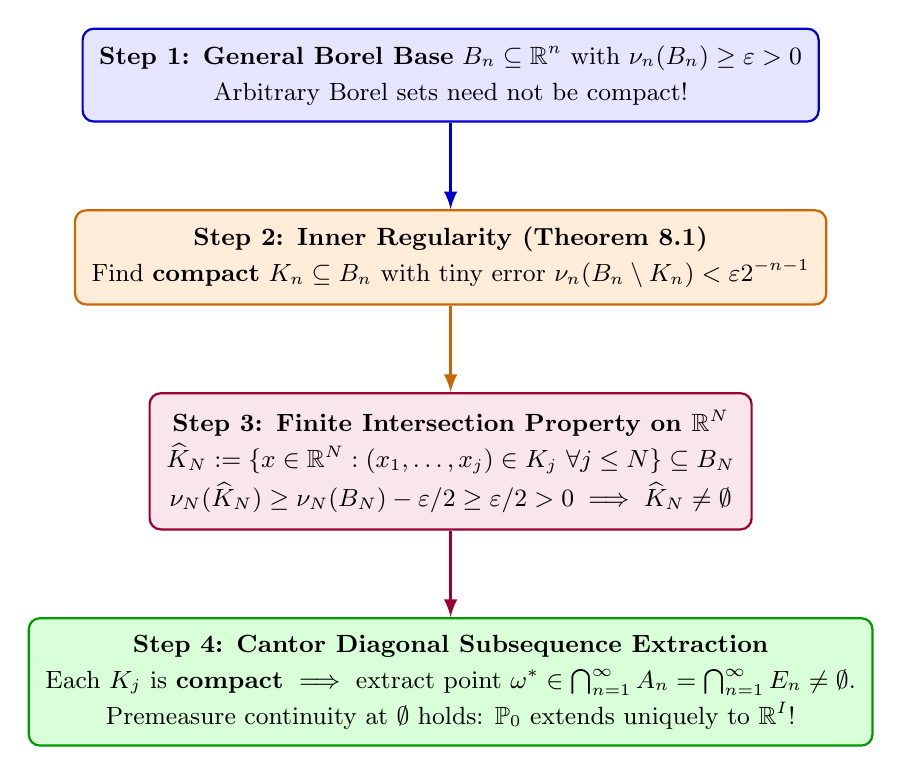
\begin{tikzpicture}[>=latex, font=\small, node distance=1.1cm]
  \node[draw=blue!80!black, fill=blue!10, rounded corners, thick, align=center, inner sep=6pt] (b1)
    {\textbf{Step 1: General Borel Base} $B_n \subseteq \mathbb{R}^n$ with $\nu_n(B_n) \ge \varepsilon > 0$\\[2pt]
     Arbitrary Borel sets need not be compact!};

  \node[draw=orange!80!black, fill=orange!15, rounded corners, thick, align=center, inner sep=6pt, below=of b1] (b2)
    {\textbf{Step 2: Inner Regularity (Theorem 8.1)}\\[2pt]
     Find \textbf{compact} $K_n \subseteq B_n$ with tiny error $\nu_n(B_n \setminus K_n) < \varepsilon 2^{-n-1}$};

  \node[draw=purple!80!black, fill=purple!10, rounded corners, thick, align=center, inner sep=6pt, below=of b2] (b3)
    {\textbf{Step 3: Finite Intersection Property on $\mathbb{R}^N$}\\[2pt]
     $\widehat{K}_N := \{x \in \mathbb{R}^N : (x_1,\dots,x_j) \in K_j\ \forall j \le N\} \subseteq B_N$\\[2pt]
     $\nu_N(\widehat{K}_N) \ge \nu_N(B_N) - \varepsilon/2 \ge \varepsilon/2 > 0 \implies \widehat{K}_N \ne \emptyset$};

  \node[draw=green!60!black, fill=green!15, rounded corners, thick, align=center, inner sep=6pt, below=of b3] (b4)
    {\textbf{Step 4: Cantor Diagonal Subsequence Extraction}\\[2pt]
     Each $K_j$ is \textbf{compact} $\implies$ extract point $\omega^* \in \bigcap_{n=1}^\infty A_n = \bigcap_{n=1}^\infty E_n \neq \emptyset$.\\[2pt]
     Premeasure continuity at $\emptyset$ holds: $\mathbb{P}_0$ extends uniquely to $\mathbb{R}^I$!};

  \draw[->, very thick, blue!80!black] (b1) -- (b2);
  \draw[->, very thick, orange!80!black] (b2) -- (b3);
  \draw[->, very thick, purple!80!black] (b3) -- (b4);
\end{tikzpicture}
\end{document}
